\chapter{Introduction}\label{ch:intro}

In this chapter we are going to describe accurately the problem and provide a possible 
solution (from the point of view of a Distributed Systems designer).\\


\section{The Problem}

The bridge has a \textbf{maximum capacity} $c \geq 1$ and a \textbf{length} $l \geq 1$. \\

Cars can send messages to adjacent cars (to the car in front and to the rear one); 
cars can also have the ability to speak with more than two other cars depending on the 
\textbf{power of their transmission medium} $p \geq 1$.\\

So basically a car can only send messages to the $p$ cars in front and 
to the $p$ cars behind. We assume that the bridge length doesn't constitute an impediment 
for the communications (so even if the bridge was very long, however, 
the cars can send messages as if they were close).\\

Moreover a car has a certain \textbf{speed} $s \geq 1 \frac{block}{s}$ that determines 
the bridge crossing time and the time to reach the first obstacle 
(another enqueued car or the bridge).\\ 

For simplicity we assume that every car has the 
same dimensions expressed in an arbitrary length scale called \textbf{block} and 
\textbf{every measure is an integer} ($s$, $l$, $c$, $p$, etc.). \\

We assume that cars can have a failure at any moment and there are only 
three types of failures:
\begin{itemize}
    \item \textbf{engine failure} (the car cannot move but can send help messages to the other cars)
    \item \textbf{link failure} (the car can move but cannot send any message)
    \item \textbf{system failure} (the car cannot move and cannot send messages)
\end{itemize}

We assume that a link failure is equivalent to a system failure cause the car cannot 
take any decision without the agreement of the others. 
In case of engine failure or system failure the car or another helping car must call 
a tow truck in order to remove the broken car 
(in this case we have to wait an \textbf{elimination time} $e$).\\

We assume that a car cannot be malicius (must follow the algorithm) but the communication 
channel isn't secure so it is exposed to a \textbf{MIM} (man in the middle) attack 
(drop messages, edit messages, message injection, ...).\\

Finally we have to consider that in a distributed system a global up-to-date state 
or a global timing cannot exist; this implies that each car can have a partial 
and \textbf{inconsistent view} of the global environment and a \textbf{time drift} 
from the global time.


\begin{figure}
    \centering
    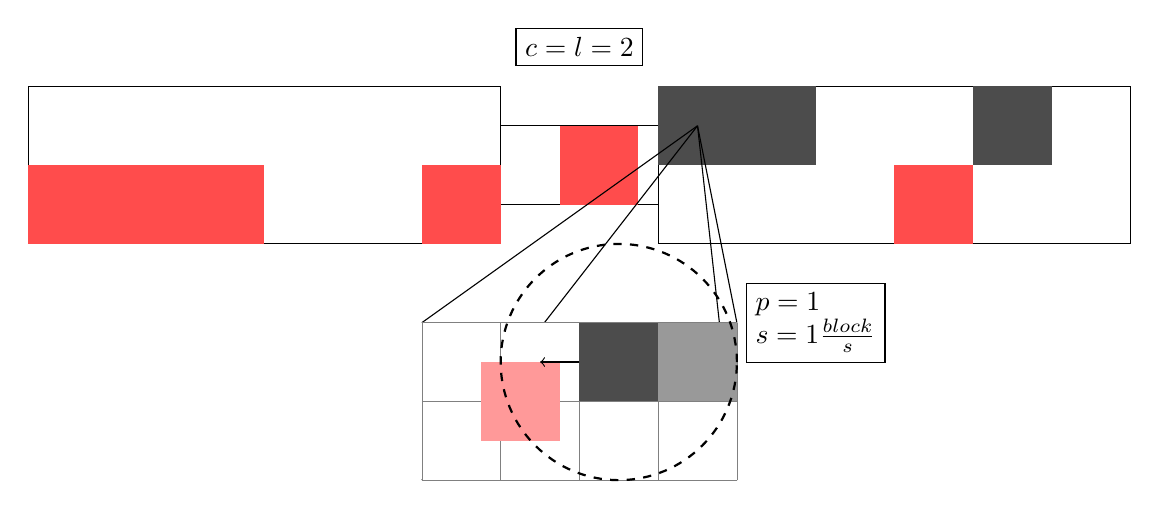
\begin{tikzpicture}
        % queues
        \draw (1,-1) rectangle (7,1);
        \draw (-7,-1) rectangle (-1,1);
        
        % bridge
        \draw (-1,-0.5) rectangle (1,0.5);
        \fill[red!70!white] (-0.25,-0.5) rectangle (0.75,0.5);
        \fill[red!70!white] (4,-1) rectangle (5,0);
        \node[draw,align=left] at (0,1.5) {$c = l = 2$};
        
        % left cars
        \fill[red!70!white] (-7,-1) rectangle (-6,0);
        \fill[red!70!white] (-6,-1) rectangle (-5,0);
        \fill[red!70!white] (-5,-1) rectangle (-4,0);
        \fill[red!70!white] (-2,-1) rectangle (-1,0);
        
        %% right cars
        \fill[black!70!white] (1,0) rectangle (2,1);
        \fill[black!70!white] (2,0) rectangle (3,1);
        \fill[black!70!white] (5,0) rectangle (6,1);
        
        \draw[black] (1.5,0.5) -- (-2, -2);
        \draw[black] (1.5,0.5) -- (2, -2);
        \draw[black] (1.5,0.5) -- (-2, -4);
        \draw[black] (1.5,0.5) -- (2, -4);

        % grid
        \fill[white]  (-2,-4) rectangle (2, -2);
        \draw[step=1cm,gray,very thin] (-2,-4) grid (2, -2);
        \fill[black!70!white] (0,-3) rectangle (1,-2);
        \fill[black!40!white] (1,-3) rectangle (2,-2);
        \fill[red!40!white] (-1.25,-3.5) rectangle (-0.25,-2.5);

        \draw[black,thick,dashed] (0.5,-2.5) circle (1.5cm);
        \node[draw,align=left] at (3,-2) {$p = 1$\\ $s = 1 \frac{block}{s}$};
        \draw[->,black] (0,-2.5) -- (-0.5, -2.5);
    \end{tikzpicture}
    \caption{Example of a possible situation} \label{fig:1}
\end{figure}


\section{Subproblems}

Following the \textit{divide et impera} philosophy now we are going to split the problem 
into some subproblems and solve them. 


\subsection{Starvation and FIFO}

Ideally a car that reaches first the queue must pass before other incoming cars (FIFO).\\

Moreover we have to consider the possibility of starvation when 
cars doesn't reach the agreement (ie. in case of a bad agorithm that falls into 
a deadlock).


\subsection{Solution}

Define the \textbf{local waiting time} $ltime$ as the time that passes between the instant when the car reaches 
the queue and the instant in which the car ends to cross the bridge. \\

Define the \textbf{global waiting time} $gtime$ as the sum of the $ltime$ of the cars.\\

If we focus on minimizing the global waiting time (maximize the throughput of the bridge) 
we implicit avoid deadlock but don't consider starvation and the FIFO constraint. 

\begin{figure}
    \centering
    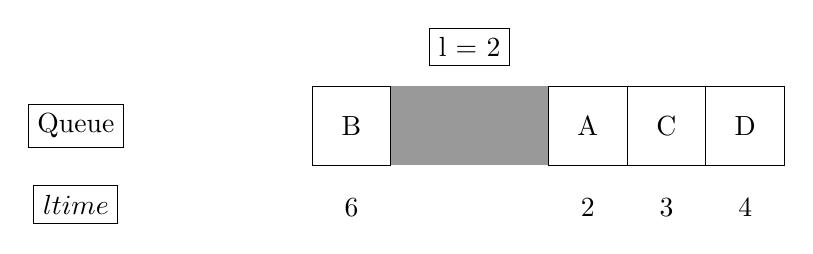
\begin{tikzpicture}
        % queues
        \draw (1,0) rectangle (2,1) node[pos=.5] {A} node[pos=.5, below=0.8cm] {2};
        \draw (2,0) rectangle (3,1) node[pos=.5] {C} node[pos=.5, below=0.8cm] {3};
        \draw (3,0) rectangle (4,1) node[pos=.5] {D} node[pos=.5, below=0.8cm] {4};
        
        \draw (-2,0) rectangle (-1,1) node[pos=.5] {B} node[pos=.5, below=0.8cm] {6};
        % bridge
        \fill[black!40!white] (-1,0) rectangle (1,1);
        \node[draw,align=left] at (0, 1.5) {l = 2};
        \node[draw,align=left] at (-5, -0.5) {$ltime$};
        \node[draw,align=left] at (-5, 0.5) {Queue};
    \end{tikzpicture}
    \caption{Minimizing global waiting time: A-C-D-B. $gtime = 15$} \label{fig:1}
\end{figure}

If on the right side we have an infinite queue then B waits forever and the 
$gtime$ is the lowest.

\begin{figure}
    \centering
    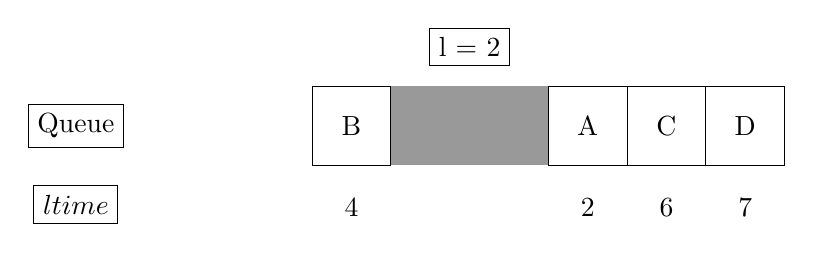
\begin{tikzpicture}
        % queues
        \draw (1,0) rectangle (2,1) node[pos=.5] {A} node[pos=.5, below=0.8cm] {2};
        \draw (2,0) rectangle (3,1) node[pos=.5] {C} node[pos=.5, below=0.8cm] {6};
        \draw (3,0) rectangle (4,1) node[pos=.5] {D} node[pos=.5, below=0.8cm] {7};
        
        \draw (-2,0) rectangle (-1,1) node[pos=.5] {B} node[pos=.5, below=0.8cm] {4};
        % bridge
        \fill[black!40!white] (-1,0) rectangle (1,1);
        \node[draw,align=left] at (0, 1.5) {l = 2};
        \node[draw,align=left] at (-5, -0.5) {$ltime$};
        \node[draw,align=left] at (-5, 0.5) {Queue};
    \end{tikzpicture}
    \caption{FIFO order: A-B-C-D. $gtime = 19$} \label{fig:1}
\end{figure}

FIFO order avoids deadlock and starvation but doesn't minimize $gtime$. 
The idea is then find the right trade off between minimizing 
$gtime$ and minimizing $ltime$ locally (starvation).

The concept of equity comes to the rescue cause 

\section{Agreement}


\section{Communications}


\section{Solution}